% UPDATED BY MARCUS SCHAGERBERG, 2023
% CREATED BY WOLFGANG AHRENDT, 2021

In the following sections, examples of a figure, an equation, a table and a source code listing  are shown.

\section{Figure}
    \begin{figure}[H]
        \centering
        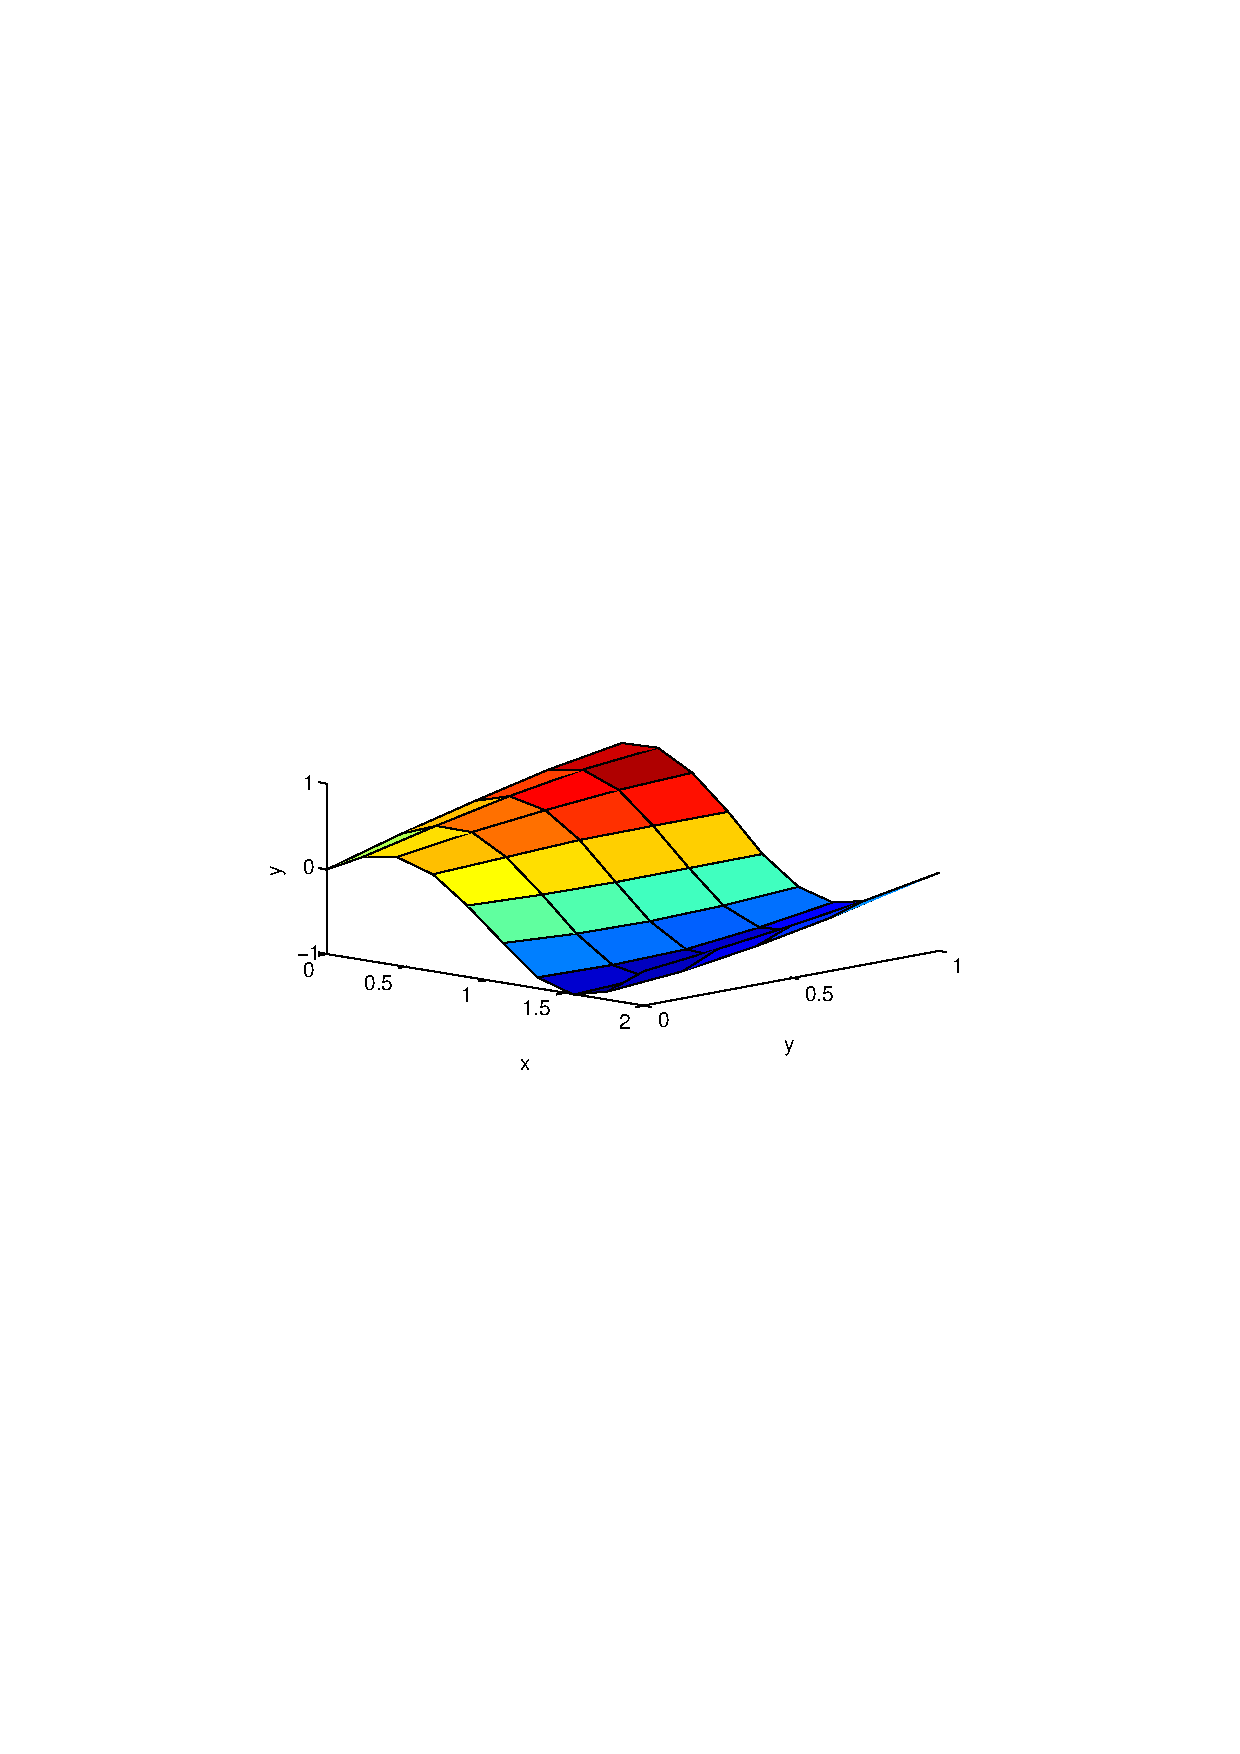
\includegraphics[width=0.45\linewidth, trim=3cm 11cm 3cm 11cm]{figures/X.pdf}
        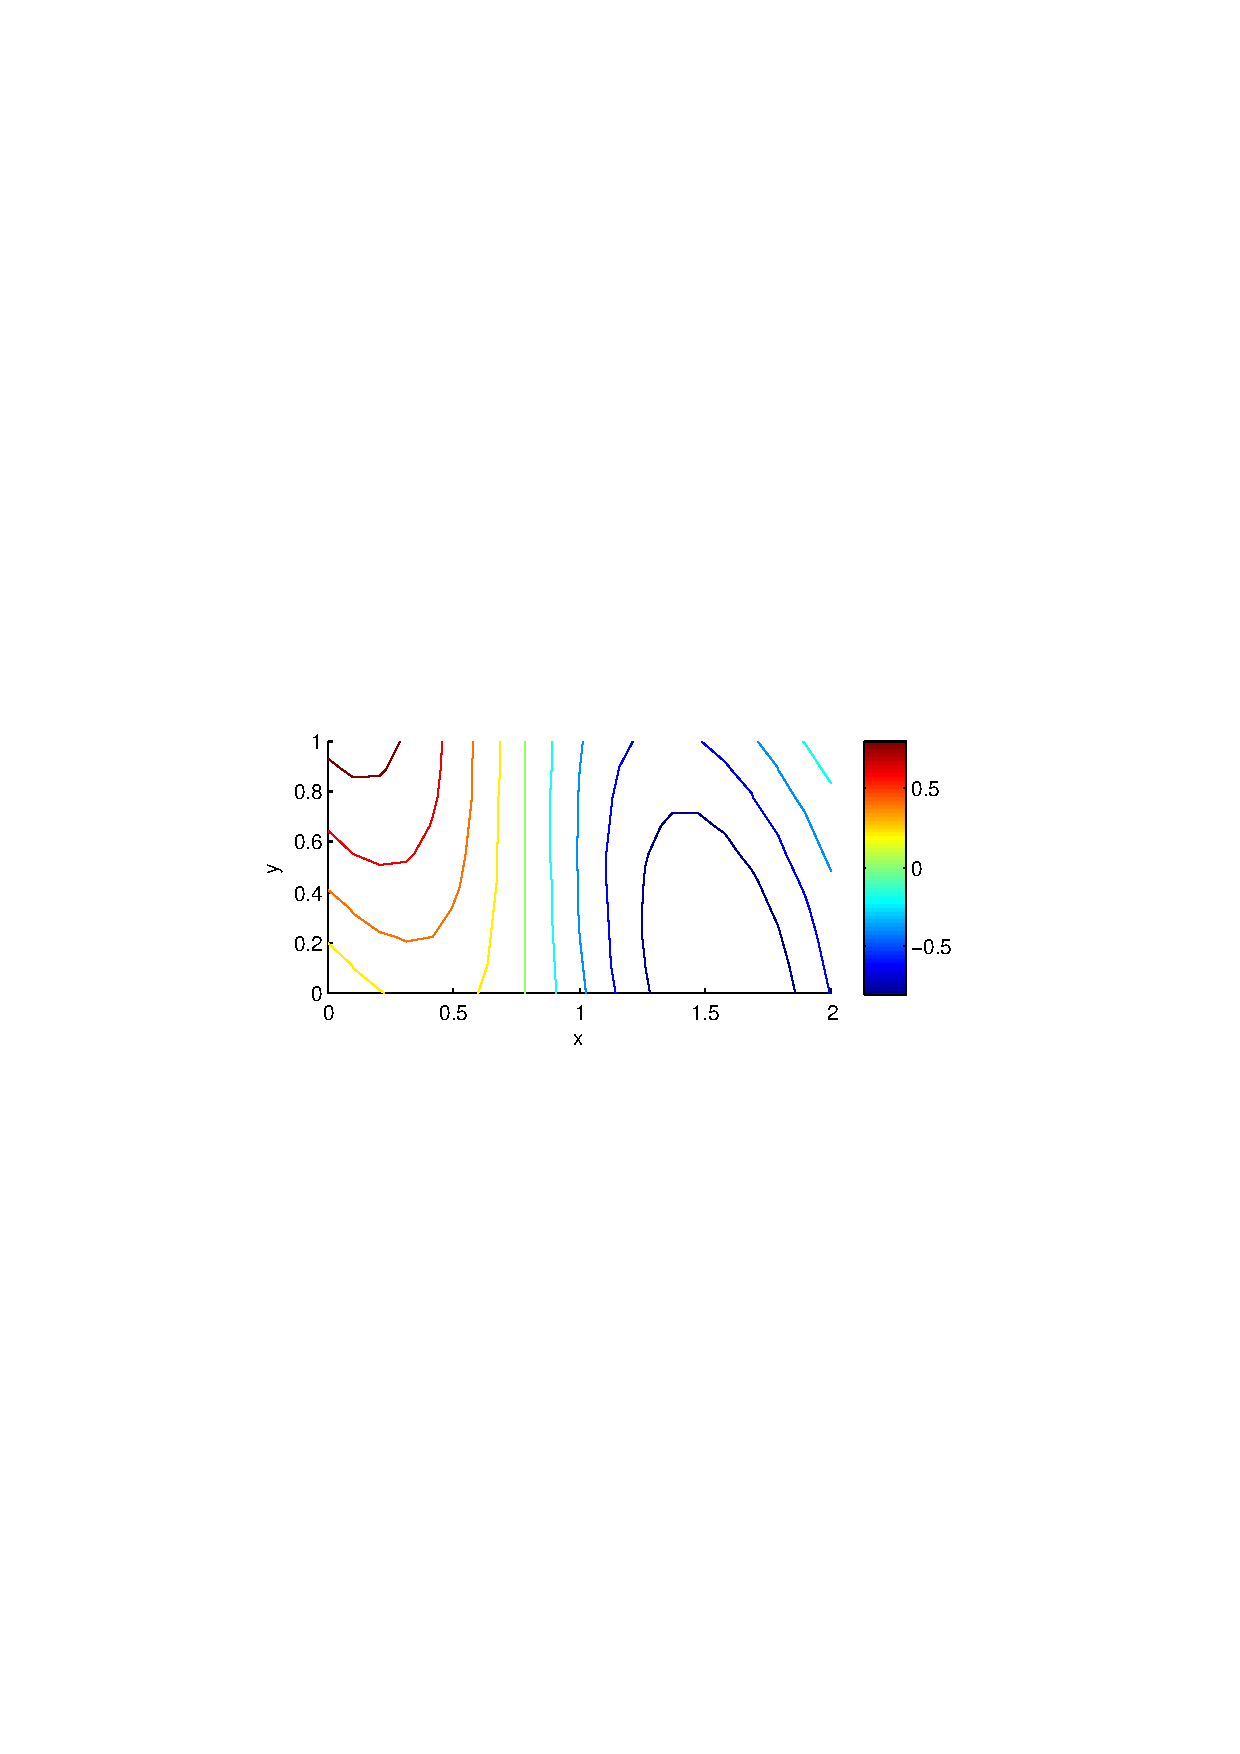
\includegraphics[width=0.45\linewidth, trim=3cm 11cm 3cm 11cm]{figures/Y.pdf}
        \caption{Surface and contour plots showing the two dimensional function $z(x,y)=\sin(x+y)\cos(2x)$.}
    \end{figure}

\section{Equation}
    \begin{equation}
        f(t)=\left\{ \begin{array}{ll}
        1,~~~~ & t< 1 \\
        t^2 & t\geq 1
        \end{array}\right.
    \end{equation}

\section{Table}
    \begin{table}[H]
        \centering
        \caption{Values of $f(t)$ for $t=0,1,\dots 5$.}
        \begin{tabular}{l|llllll} \hline\hline
            $t$ & 0 & 1 & 2 & 3 & 4 & 5 \\ \hline
            $f(t)$ & 1 & 1 & 4 & 9 & 16 & 25 \\ \hline\hline
        \end{tabular}
    \end{table}


\section{Source code listing}
\begin{minted}[frame=single]{matlab}
    % Generate x- and y-nodes
    x=linspace(0,1); y=linspace(0,1);
    
    % Calculate z=f(x,y)
    for i=1:length(x)
     for j=1:length(y)
      z(i,j)=x(i)+2*y(j);
     end
    end
\end{minted}
